\documentclass[UTF8,a4paper,12pt]{ctexart}

\usepackage{geometry}
\usepackage{booktabs}
\usepackage{longtable}
\usepackage{array}
\usepackage{hyperref}
\usepackage{xcolor}
\usepackage{listings}
\usepackage{caption}
\usepackage{graphicx}

\geometry{left=2.5cm,right=2.5cm,top=2.5cm,bottom=2.5cm}
\hypersetup{colorlinks=true,linkcolor=blue,urlcolor=blue,citecolor=blue}
\captionsetup{font=small}

\lstset{
  basicstyle=\ttfamily\small,
  breaklines=true,
  columns=fullflexible,
  frame=single,
  backgroundcolor=\color{gray!6}
}

\title{Project 2：AISHELL-1 约 10 小时子集中文语音识别系统实验报告}
\author{林子淳 524030910206}
\date{\today}

\begin{document}
\maketitle

\begin{abstract}
本实验围绕 AISHELL-1 普通话语音数据构建完整 LVCSR 系统，重点完成从数据准备、特征提取、语言模型训练、GMM-HMM 声学模型训练、DNN-HMM 系统构建，到最终解码与 CER/WER 评估的闭环。传统系统使用 Kaldi recipe 实现，包括 mono、tri1、tri2、tri3a、tri4a、tri5a 以及 nnet3 TDNN；此外，为了对比预训练端到端模型，本实验额外实现了 Whisper-small 的测试集 baseline 解码和基于约 10 小时训练集的监督微调。最终主要指标以 CER 为准，WER 作为参考。Kaldi TDNN 在测试集上达到 17.39\% CER；Whisper-small 预训练模型微调前测试集 CER 为 26.77\%，微调并进行统一文本规范化评分后测试集 CER 为 8.45\%，显著优于传统 Kaldi 系统。
\end{abstract}

\section{实验目标与任务理解}

本次 Project 2 的目标是理解中文大词汇连续语音识别系统从原始音频和标注文本到最终解码结果的完整流程。根据作业要求，本实验重点关注以下内容：

\begin{itemize}
  \item 按 Kaldi 数据规范准备 \texttt{wav.scp}、\texttt{text}、\texttt{utt2spk}、\texttt{spk2utt}、词表、发音词典与语言模型文本；
  \item 提取 MFCC+pitch 特征并计算 CMVN；
  \item 训练传统 GMM-HMM 系统，理解其在初始对齐、上下文相关建模、特征变换中的作用；
  \item 在 GMM-HMM 对齐基础上训练 DNN-HMM 系统，即 Kaldi nnet3 TDNN；
  \item 在同一数据划分上额外训练 Whisper-small，并严格报告预训练模型微调前后的性能差异；
  \item 使用 CER 作为主要指标，WER 作为参考指标，并明确每个结果来自的模型与解码目录。
\end{itemize}

\section{实验环境}

本实验在本地项目目录中完成：

\begin{lstlisting}
/inspire/hdd/project/robot-reasoning/xiangyushun-p-xiangyushun/zichun/speech/speech/project2_asr
\end{lstlisting}

Kaldi 使用本地源码构建，路径为：

\begin{lstlisting}
/inspire/hdd/project/robot-reasoning/xiangyushun-p-xiangyushun/zichun/speech/speech/downloads/kaldi
\end{lstlisting}

主要环境配置如下：

\begin{itemize}
  \item Kaldi：本地编译版本；
  \item BLAS：OpenBLAS；
  \item OpenFST：Kaldi tools 中本地构建版本；
  \item CUDA：Kaldi 编译启用 CUDA，\texttt{CUDA = true}，\texttt{WITH\_CUDADECODER = true}；
  \item GPU：NVIDIA GeForce RTX 4090；
  \item Kaldi GPU 架构参数：\texttt{-gencode arch=compute\_89,code=sm\_89}；
  \item Python：3.11；
  \item Whisper 相关库：PyTorch 2.6.0+cu124、Transformers 4.40.0、librosa、soundfile、OpenCC。
\end{itemize}

需要说明的是，Kaldi 的 GMM-HMM 训练阶段主要在CPU上完成；nnet3 TDNN 和 Whisper 训练可使用 GPU。TDNN 训练脚本配置为单 GPU job，以避免 RTX 4090 上多个 GPU 训练任务同时运行导致显存竞争。

\section{数据集与数据准备}

\subsection{数据划分}

本实验使用 AISHELL-1 子集，并保持固定划分。数据目录结构如下：

\begin{lstlisting}
project2_asr/
  data_aishell/
    transcript/aishell_transcript_v0.8.txt
    wav/
      train/
      dev/
      test/
  resource_aishell/
    lexicon.txt
    speaker.info
\end{lstlisting}

各集合统计如表 \ref{tab:data-stat} 所示。

\begin{table}[htbp]
  \centering
  \caption{数据集划分统计}
  \label{tab:data-stat}
  \begin{tabular}{lrr}
    \toprule
    集合 & 语音条数 & 时长说明 \\
    \midrule
    Train & 8,000 & 约 10.0 小时，单条均不超过 10 秒 \\
    Dev & 14,326 & 约 18.1 小时 \\
    Test & 7,176 & 约 10.0 小时 \\
    Total & 29,502 & 约 38.1 小时 \\
    \bottomrule
  \end{tabular}
\end{table}

训练集使用约 10 小时普通话语音，符合任务设计；dev/test 保持 AISHELL-1 对应集合完整，以便稳定评估模型泛化性能。

\subsection{Kaldi 数据规范}

数据准备阶段生成并验证以下 Kaldi 标准文件：

\begin{itemize}
  \item \texttt{wav.scp}：记录 utterance id 到音频路径的映射；
  \item \texttt{text}：记录 utterance id 到转写文本的映射；
  \item \texttt{utt2spk}：记录 utterance 到 speaker 的映射；
  \item \texttt{spk2utt}：由 \texttt{utt2spk} 反向生成；
  \item \texttt{lexicon.txt}：发音词典；
  \item 语言模型文本：用于训练 n-gram 语言模型。
\end{itemize}

对应数据目录为：

\begin{lstlisting}
data/train
data/dev
data/test
data/lang
data/lang_test
\end{lstlisting}

特征清单数量与划分一致：

\begin{lstlisting}
data/train/feats.scp   8000 entries
data/dev/feats.scp    14326 entries
data/test/feats.scp    7176 entries
\end{lstlisting}

\section{传统 Kaldi LVCSR 系统}

\subsection{特征提取}

Kaldi 系统使用 MFCC+pitch 特征，并为 train、dev、test 分别计算 CMVN 统计量。MFCC 提供短时谱包络特征，pitch 特征补充基频与声调相关信息；对于普通话识别，pitch 信息对声调区分有实际意义。CMVN 用于减小说话人、录音设备和通道差异带来的均值方差偏移。

\subsection{语言模型训练}

语言模型使用训练文本构建，输出到 \texttt{data/lang\_test} 相关目录。GMM-HMM 和 TDNN 解码均依赖词图和语言模型，最终解码图由声学模型、发音词典、上下文依赖和语言模型组合得到。

\subsection{GMM-HMM 训练流程}

GMM-HMM 在本实验中不是附属步骤，而是传统 ASR 系统的重要基础。其作用包括：

\begin{itemize}
  \item 训练初始单音素模型，获得可用的初始对齐；
  \item 逐步引入上下文相关三音素模型，提高声学建模能力；
  \item 使用 LDA、MLLT、SAT 等技术改进特征空间与说话人适应；
  \item 为后续 DNN-HMM 提供较可靠的帧级对齐。
\end{itemize}

本实验完成的主要 GMM-HMM 阶段包括：

\begin{itemize}
  \item \texttt{mono}：单音素模型；
  \item \texttt{tri1}：上下文相关三音素模型；
  \item \texttt{tri2}：进一步增强的三音素模型；
  \item \texttt{tri3a}：加入 LDA/MLLT；
  \item \texttt{tri4a}：加入 SAT/fMLLR；
  \item \texttt{tri5a}：后续增强系统。
\end{itemize}

\subsection{DNN-HMM：nnet3 TDNN}

在 GMM-HMM 对齐基础上，本实验训练 Kaldi nnet3 TDNN。TDNN 通过时间延迟结构利用上下文帧信息，相比 GMM-HMM 具有更强的非线性声学建模能力。其训练依赖前面 GMM-HMM 阶段提供的对齐和高分辨率特征，体现了传统混合式 ASR 系统中 ``GMM-HMM 提供对齐，DNN-HMM 提升声学模型'' 的典型流程。

最终 TDNN 模型位置为：

\begin{lstlisting}
project2_asr/exp/nnet3/tdnn_sp/final.mdl
\end{lstlisting}

主要解码目录为：

\begin{lstlisting}
project2_asr/exp/nnet3/tdnn_sp/decode_dev
project2_asr/exp/nnet3/tdnn_sp/decode_test
\end{lstlisting}

\section{Whisper-small 预训练模型与监督微调}

\subsection{引入 Whisper 的原因}

作业鼓励尝试不同范式的神经网络模型，若使用预训练权重进行 SFT需要严格报告微调前后的测试集性能差异。因此，本实验在 Kaldi 系统之外额外实现 Whisper-small 实验，用同一份 AISHELL-1 数据划分进行 baseline 解码与监督微调。

Whisper 实验目录为：

\begin{lstlisting}
project2_asr/whisper
\end{lstlisting}

主要脚本包括：

\begin{itemize}
  \item \texttt{prepare\_whisper\_data.py}：将 Kaldi 数据格式转换为 JSONL；
  \item \texttt{train\_whisper.py}：Whisper-small 监督微调；
  \item \texttt{decode\_whisper.py}：Whisper 解码；
  \item \texttt{score\_whisper.py}：CER/WER 评分；
  \item \texttt{run\_whisper\_baseline.sh}：预训练模型 baseline 解码；
  \item \texttt{run\_whisper\_finetune.sh}：微调与 dev/test 解码。
\end{itemize}

\subsection{数据转换}

Whisper 直接复用 Kaldi 的 \texttt{data/train}、\texttt{data/dev}、\texttt{data/test}，保证与 Kaldi 实验使用相同训练、验证与测试集合。转换后的 JSONL 文件包括：

\begin{lstlisting}
whisper/data/train.jsonl
whisper/data/dev.jsonl
whisper/data/test.jsonl
\end{lstlisting}

每条记录包含 utterance id、音频绝对路径和文本：

\begin{lstlisting}
{"utt_id": "...", "audio": "/abs/path.wav", "text": "中文转写"}
\end{lstlisting}

\subsection{微调方式}

由于当前运行环境中 Hugging Face Trainer 相关依赖会触发 \texttt{sklearn/numpy} 二进制兼容问题，且已有 \texttt{flash\_attn} 扩展与当前 PyTorch 版本不兼容，本实验采用纯 PyTorch 训练循环实现 Whisper-small 微调。该实现与 Trainer 的核心优化目标一致，均为 Whisper encoder-decoder 的序列到序列交叉熵训练。

微调配置如下：

\begin{itemize}
  \item 预训练模型：\texttt{openai/whisper-small}；
  \item 语言：Chinese；
  \item 任务：transcribe；
  \item 优化器：AdamW；
  \item 学习率：$1\times10^{-5}$；
  \item 最大训练步数：4000；
  \item batch size：2；
  \item gradient accumulation：4；
  \item 等效 batch size：约 8；
  \item 使用 AMP 与 gradient checkpointing 控制显存。
\end{itemize}

训练过程中每 500 step 进行一次 dev CER 评估，观察到的采样 dev CER 如表 \ref{tab:whisper-train-curve} 所示。

\begin{table}[htbp]
  \centering
  \caption{Whisper-small 微调过程中的 dev CER}
  \label{tab:whisper-train-curve}
  \begin{tabular}{rr}
    \toprule
    Step & Dev CER(\%) \\
    \midrule
    500 & 16.37 \\
    1000 & 14.85 \\
    1500 & 13.83 \\
    2000 & 14.25 \\
    2500 & 13.09 \\
    3000 & 13.16 \\
    3500 & 12.28 \\
    4000 & 13.30 \\
    \bottomrule
  \end{tabular}
\end{table}

图 \ref{fig:whisper-dev-curve} 进一步展示了 Whisper-small 微调过程中 dev CER 的变化趋势。

\begin{figure}[htbp]
  \centering
  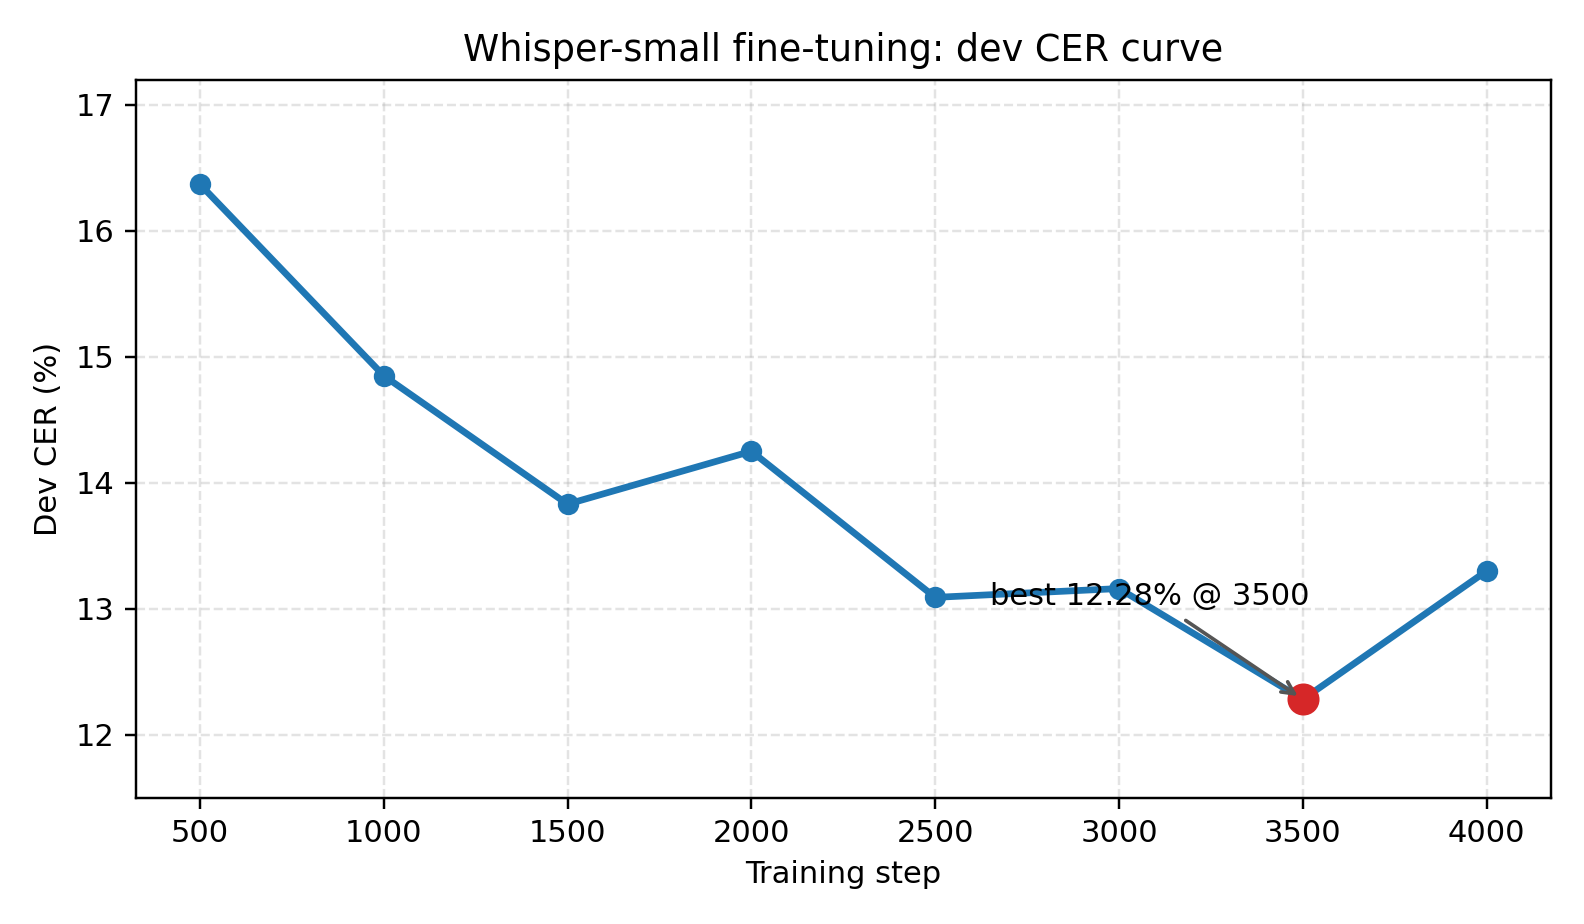
\includegraphics[width=0.82\textwidth]{report_figures/whisper_dev_cer_curve.png}
  \caption{Whisper-small 微调过程中 dev CER 的变化趋势。曲线显示模型在 3500 step 附近达到采样 dev 评估最优值，之后略有波动。}
  \label{fig:whisper-dev-curve}
\end{figure}

最终模型位置为：
\begin{lstlisting}
project2_asr/exp/whisper_small/finetuned
\end{lstlisting}

训练过程中 dev 采样评估最优 checkpoint 为：

\begin{lstlisting}
project2_asr/exp/whisper_small/finetuned/best
\end{lstlisting}

\section{评估方法}

\subsection{评价指标}

根据作业要求，本实验以 CER 为主要指标，WER 为参考指标。对于中文识别，字符级错误率更能稳定反映识别质量，因为中文词切分方式会显著影响 WER。Kaldi 的 CER 结果来自 \texttt{scoring\_kaldi} 下的 \texttt{cer\_*} 文件；Whisper 的 CER/WER 由 \texttt{score\_whisper.py} 计算。

CER 计算方式为：

\[
\mathrm{CER} = \frac{S + D + I}{N} \times 100\%,
\]

其中 $S$、$D$、$I$ 分别为替换、删除和插入错误数，$N$ 为参考文本字符数。

\subsection{文本规范化}

为保证 Whisper 输出与中文参考文本格式一致，最终 Whisper 结果额外使用统一文本规范化评分。规范化同时作用于 reference 和 hypothesis，包括：

\begin{itemize}
  \item 繁体转简体；
  \item Unicode NFKC 规范化；
  \item 去除标点符号和符号类字符；
  \item 去除空白字符；
  \item 英文字母小写化。
\end{itemize}

Whisper 评分脚本按字符级统一计算，因此 Whisper 表中的 WER 与 CER 数值一致，与 Kaldi 的词级 WER 口径不同，仅作为参考。

该处理避免将 ``因為/因为''、``儲備/储备''、全角半角差异或标点差异计为识别错误。规范化评分会在最佳结果目录中生成与该模型输出一致的 \texttt{test_filt.txt} 和 \texttt{test_filt.chars.txt}，同时保留 \texttt{hyp_filt.txt} 与 \texttt{hyp_filt.chars.txt} 便于核查预测文本和参考文本格式。规范化脚本为：

\begin{lstlisting}
project2_asr/whisper/score_whisper.py
\end{lstlisting}

\section{实验结果}

\subsection{Kaldi GMM-HMM 与 TDNN 结果}

GMM-HMM 系统测试集结果如表 \ref{tab:gmm-results} 所示。

\begin{table}[htbp]
  \centering
  \caption{GMM-HMM 测试集结果}
  \label{tab:gmm-results}
  \begin{tabular}{lrr}
    \toprule
    模型 & WER(\%) & CER(\%) \\
    \midrule
    tri2 & 43.56 & 28.35 \\
    tri3a & 41.36 & 25.87 \\
    tri4a & 36.60 & 20.89 \\
    tri5a & 37.99 & 22.43 \\
    \bottomrule
  \end{tabular}
\end{table}

其中最佳 GMM-HMM 为 \texttt{tri4a}，测试集 CER 为 20.89\%。\texttt{tri5a} 相比 \texttt{tri4a} 未见提升，推测在约 10 小时小数据量下，后续特征或说话人自适应变换可能出现过拟合或估计不稳定。nnet3 TDNN 结果如表 \ref{tab:tdnn-results} 所示。

\begin{table}[htbp]
  \centering
  \caption{Kaldi nnet3 TDNN 结果}
  \label{tab:tdnn-results}
  \begin{tabular}{lrrl}
    \toprule
    集合 & WER(\%) & CER(\%) & 解码目录 \\
    \midrule
    dev & 30.40 & 15.14 & \texttt{exp/nnet3/tdnn\_sp/decode\_dev} \\
    test & 33.14 & 17.39 & \texttt{exp/nnet3/tdnn\_sp/decode\_test} \\
    \bottomrule
  \end{tabular}
\end{table}

可以看到，TDNN 相比最佳 GMM-HMM 将测试集 CER 从 20.89\% 降至 17.39\%，说明 DNN-HMM 的声学建模能力优于传统 GMM-HMM。

\subsection{Whisper-small 结果}

Whisper-small 的结果如表 \ref{tab:whisper-results} 所示。由于 Whisper 使用预训练权重，本实验严格报告了微调前 baseline 和微调后结果。

\begin{table}[htbp]
  \centering
  \caption{Whisper-small 测试集结果}
  \label{tab:whisper-results}
  \begin{tabular}{lrrl}
    \toprule
    设置 & WER(\%) & CER(\%) & 结果目录 \\
    \midrule
    预训练 baseline & 26.77 & 26.77 & \texttt{exp/whisper\_small/baseline\_decode\_test} \\
    微调 final，原始评分 & 8.47 & 8.47 & \texttt{exp/whisper\_small/decode\_test} \\
    微调 final，规范化评分 & 8.45 & 8.45 & \texttt{exp/whisper\_small/decode\_test\_norm} \\
    微调 best，规范化评分 & 8.53 & 8.53 & \texttt{exp/whisper\_small/decode\_test\_best\_norm} \\
    \bottomrule
  \end{tabular}
\end{table}

微调后的 final checkpoint 在规范化评分下测试集 CER 为 8.45\%，是本实验最终推荐提交的 Whisper 结果。虽然训练过程中采样 dev 评估最优 checkpoint 在完整 dev 集上取得更低 CER（7.62\%），但其测试集 CER 为 8.53\%，略差于 final checkpoint 的 8.45\%。因此最终结果采用：

\begin{figure}[htbp]
  \centering
  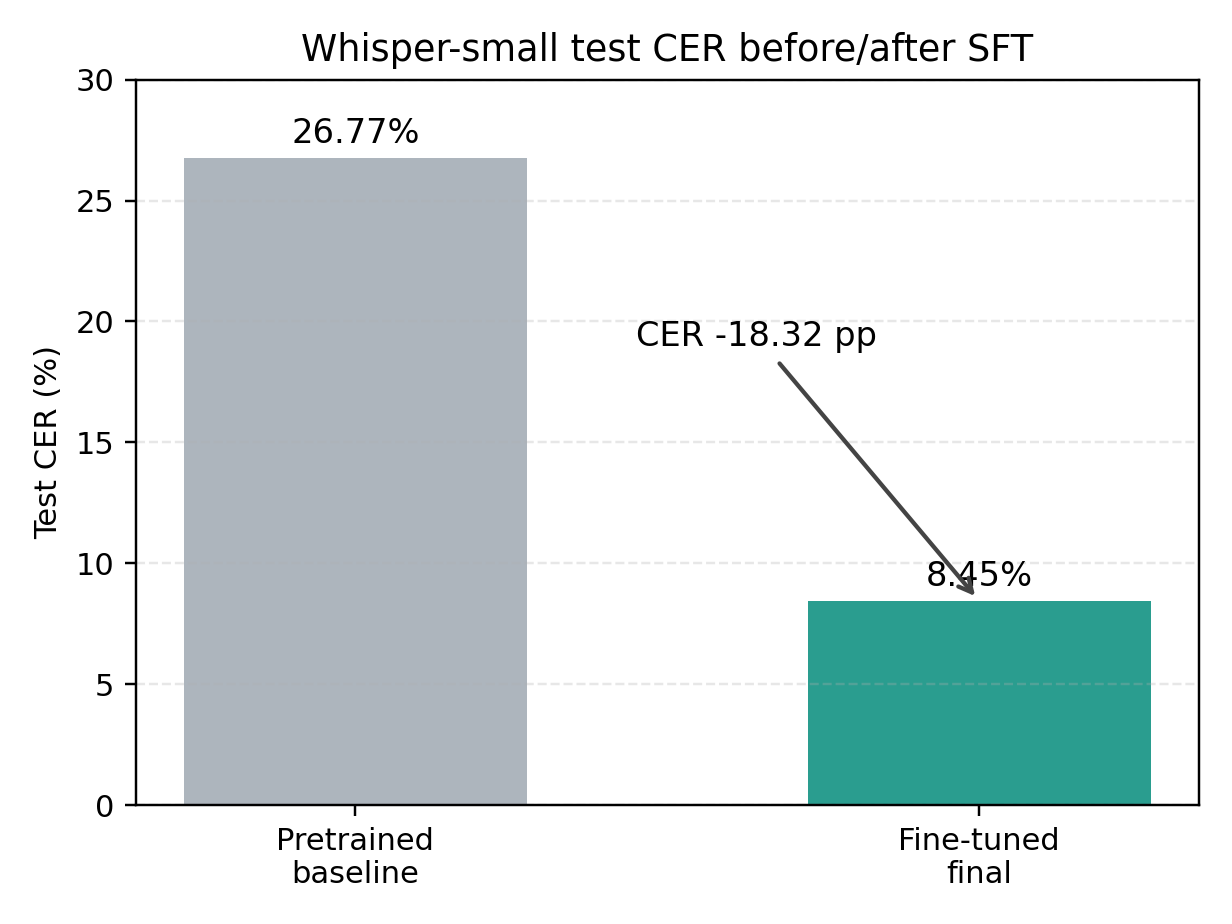
\includegraphics[width=0.62\textwidth]{report_figures/whisper_sft_gain.png}
  \caption{Whisper-small 在测试集上的微调前后 CER 对比。微调后 CER 从 26.77\% 降至 8.45\%，说明监督微调对本任务贡献显著。}
  \label{fig:whisper-sft-gain}
\end{figure}

\begin{lstlisting}
model: project2_asr/exp/whisper_small/finetuned
decode: project2_asr/exp/whisper_small/decode_test_norm
test CER: 8.45%
\end{lstlisting}

\subsection{最终模型对比}

最终主要模型测试集结果汇总如表 \ref{tab:final-compare} 所示。

\begin{table}[htbp]
  \centering
  \caption{最终测试集结果对比}
  \label{tab:final-compare}
  \begin{tabular}{lrr}
    \toprule
    模型 & WER(\%) & CER(\%) \\
    \midrule
    GMM-HMM best tri4a & 36.60 & 20.89 \\
    Kaldi nnet3 TDNN & 33.14 & 17.39 \\
    Whisper-small 预训练 baseline & 26.77 & 26.77 \\
    Whisper-small 微调 final，规范化评分 & 8.45 & 8.45 \\
    \bottomrule
  \end{tabular}
\end{table}

从结果看，Whisper-small 预训练模型不经微调时并不优于 Kaldi TDNN，主要错误包括繁简差异、同音字替换和领域文本不匹配；但在约 10 小时 AISHELL-1 训练子集上进行监督微调后，其测试集 CER 明显降低到 8.45\%，显著优于 Kaldi TDNN 的 17.39\%。这说明预训练模型具有较强迁移能力，但作业要求中的微调前后对比是必要的，否则无法判断 SFT 的实际贡献。

\begin{figure}[htbp]
  \centering
  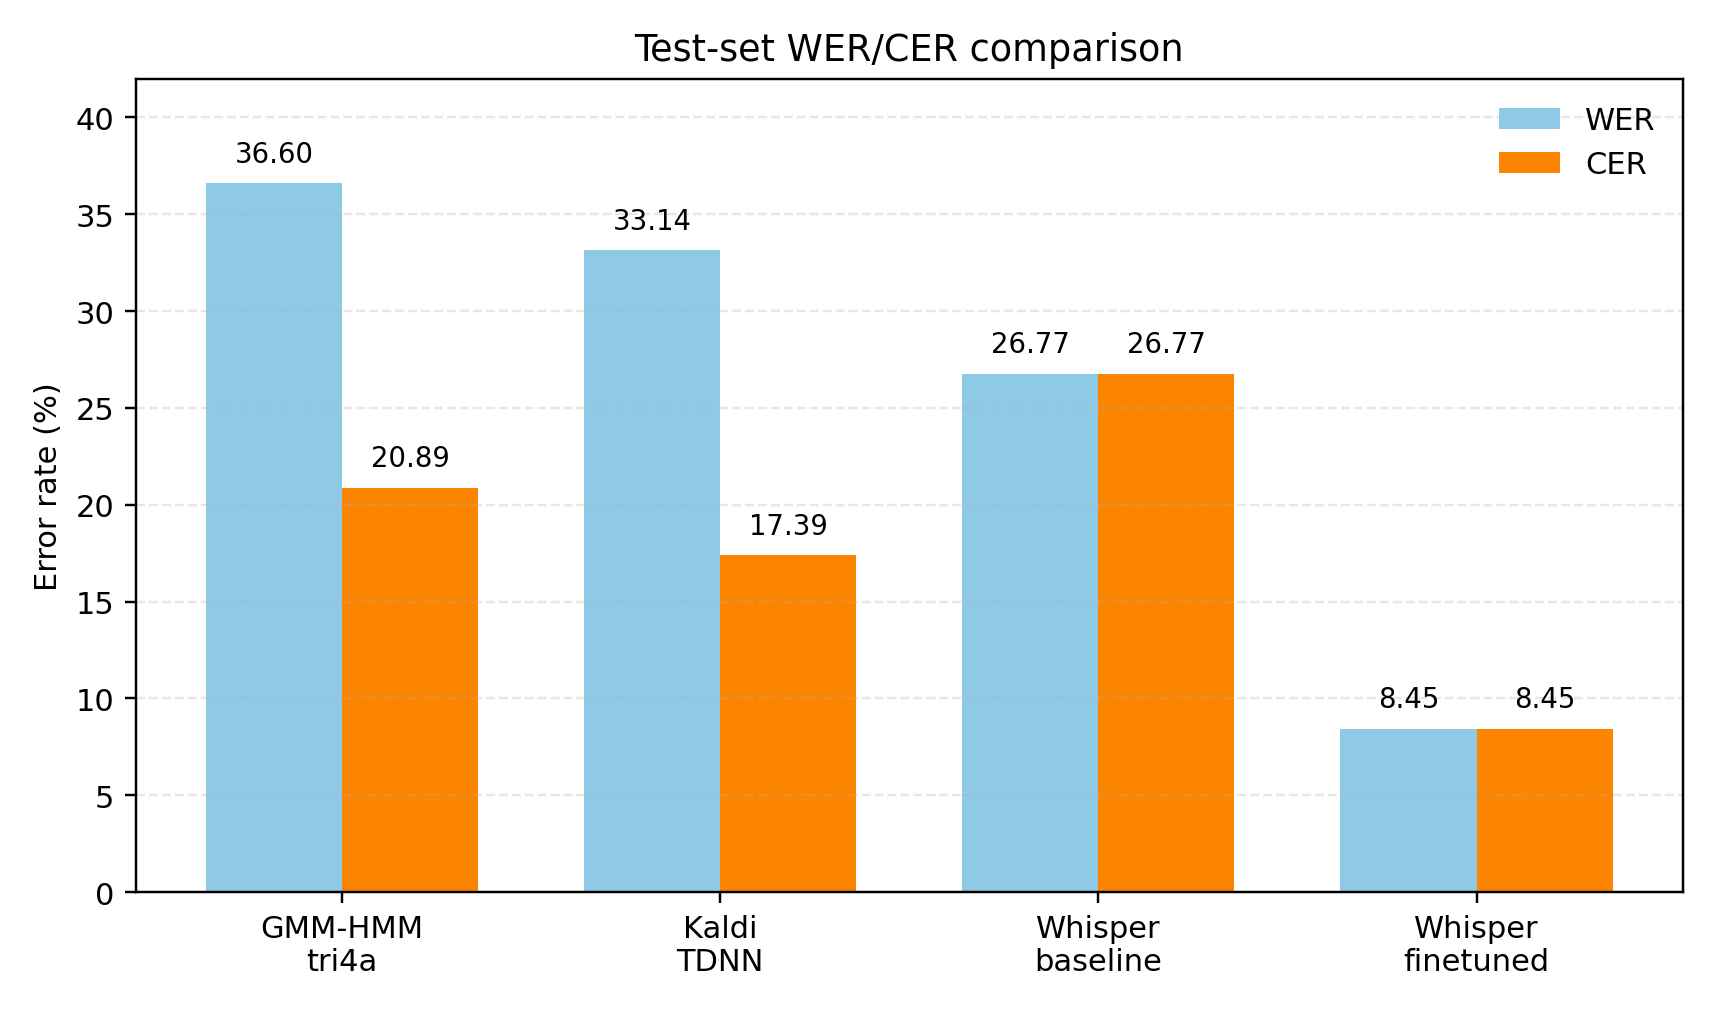
\includegraphics[width=0.9\textwidth]{report_figures/test_error_comparison.png}
  \caption{主要模型在测试集上的 WER 与 CER 对比。Whisper-small 微调后在 CER 上明显优于 GMM-HMM 与 Kaldi TDNN。}
  \label{fig:test-error-comparison}
\end{figure}

\section{复现方式}

\subsection{Kaldi 完整 recipe}

从项目目录运行：

\begin{lstlisting}
cd /inspire/hdd/project/robot-reasoning/xiangyushun-p-xiangyushun/zichun/speech/speech/project2_asr
./run.sh
\end{lstlisting}

若 GMM-HMM 对齐和高分辨率特征已经存在，仅恢复 TDNN 阶段，可运行：

\begin{lstlisting}
cd /inspire/hdd/project/robot-reasoning/xiangyushun-p-xiangyushun/zichun/speech/speech/project2_asr
. ./path.sh
local/nnet3/run_tdnn.sh
\end{lstlisting}

\subsection{Whisper baseline、微调与评分}

准备 Whisper JSONL：

\begin{lstlisting}
cd /inspire/hdd/project/robot-reasoning/xiangyushun-p-xiangyushun/zichun/speech/speech/project2_asr
python whisper/prepare_whisper_data.py
\end{lstlisting}

运行预训练 baseline：

\begin{lstlisting}
bash whisper/run_whisper_baseline.sh openai/whisper-small 8
\end{lstlisting}

运行 Whisper-small 微调和 dev/test 解码：

\begin{lstlisting}
bash whisper/run_whisper_finetune.sh openai/whisper-small
\end{lstlisting}

对已有 final 解码结果执行规范化评分：

\begin{lstlisting}
python whisper/score_whisper.py \
  --ref exp/whisper_small/decode_test/ref.txt \
  --hyp exp/whisper_small/decode_test/hyp.txt \
  --out-dir exp/whisper_small/decode_test_norm
\end{lstlisting}

对训练过程中 best checkpoint 进行完整 dev/test 解码：

\begin{lstlisting}
bash whisper/run_whisper_best_decode.sh exp/whisper_small/finetuned/best 4
\end{lstlisting}

\section{问题处理与实现细节}

实验中遇到并解决了若干实现问题：

\begin{itemize}
  \item 部分测试集 WAV 文件为 0 字节，已从原始 AISHELL-1 speaker tar 包重新解压修复；
  \item Kaldi 数据校验中中文字符会触发 non-print 检查问题，相关数据处理脚本已按中文任务需求调整；
  \item TDNN 初始训练曾出现 egs archive 数量与最终 job 数不匹配的问题，已将 \texttt{num\_jobs\_final} 调整到合理范围；
  \item 单卡 RTX 4090 上多 GPU job 并发曾导致显存压力，TDNN 训练改为单 GPU job；
  \item Whisper 环境中 \texttt{flash\_attn} 与 PyTorch 存在 ABI 不兼容，训练和解码脚本中禁用其自动加载路径；
  \item Whisper 训练中手动将 input features 转为 float16 曾导致卷积层输入与 bias 类型不一致，修复为输入保持 float32，由 AMP/autocast 自动处理混合精度；
  \item Whisper 评分加入繁简统一和标点清洗，使中文 CER 更符合任务中 ``预测结果和参考文本格式一致'' 的要求。
\end{itemize}

\section{结论}

本实验完成了作业要求的完整 ASR 系统构建流程。Kaldi GMM-HMM 系统提供了传统 ASR 基线和 DNN-HMM 所需对齐；nnet3 TDNN 相比 GMM-HMM 进一步降低测试集 CER，体现了神经声学模型的优势。在额外的 Whisper-small 实验中，预训练模型未经微调时测试集 CER 为 26.77\%，而在相同约 10 小时训练集上微调后，规范化测试集 CER 降至 8.45\%，显著优于 Kaldi TDNN。

\end{document}
